\documentclass[hyperref={unicode=true}]{beamer}

\usepackage[utf8]{inputenc}
\usepackage[english,russian]{babel}
\usepackage{../clrscode3e} 
\usepackage{xcolor}
\usepackage{pstricks, pst-tree, pst-node}
\usepackage{graphics}

%\usepackage{beamerthemesplit}

\AtBeginSubsection[]
{
  \begin{frame}<beamer>{Раздел}
    \tableofcontents[currentsection,currentsubsection]
  \end{frame}
}

\newtheorem{rtheorem}{Теорема}
\title{Декартовы деревья}
\subtitle{Дискретный анализ 2012/13}
\author{Андрей Калинин, Татьяна Романова}
\date{1 октября 2012\,г. }
\usetheme{default}
\usefonttheme[onlymath]{serif}


\begin{document}
\psset{levelsep=1cm, treesep=1cm, linewidth=0.5pt, levelsep=30pt}
\newcommand{\tnd}[1]{\Tcircle{\makebox[5mm][c]{#1}}}
\newcommand{\nilnd} {\Tp[edge=none]}
\newcommand{\rednd}[1]{\Tcircle[linecolor=red!30, %
    fillstyle=solid, fillcolor=red!30] {\makebox[5mm][c]{#1}}}
\newcommand{\blacknd}[1]{\Tcircle[linecolor=black!20, %
    fillstyle=solid, fillcolor=black!20]{\makebox[5mm][c]{#1}}}

\frame {\titlepage}

\frame
{
  \frametitle{Литература}

  \begin{itemize}
  \item Оригинальная статья: Randomized Search Trees, Siedel, Aragon. http://people.ischool.berkeley.edu/~aragon/pubs/rst96.pdf 
  \item E-maxx Максима Иванова, статья про декартовы деревья: http://e-maxx.ru/algo/treap
  \item Посты на habrahabr'е: http://habrahabr.ru/post/101818/ и т.\,п.
  \end{itemize}
}


\section{Рандомизированные деревья поиска}
\subsection{Характерные свойства}

\frame
{
  \frametitle{Проблемы обычных деревьев}
  \begin{itemize}
    \item Бинарное дерево поиска при добавлении упорядоченных данных вырождается в линейный список.
    \item Способы балансировки (avl, красно-черные, 2-3-деревья) сложно реализовать.
    \item Нет быстрых операций слияния двух деревьев или разделения по ключу.
  \end{itemize}
}

\frame
{
  \frametitle{Рандомизированные деревья}
  \begin{itemize}
    \item Разные подходы:
       \begin{itemize}
         \item Случайное поведение алгоритма: иногда вставляем в лист, иногда в середину дерева (http://habrahabr.ru/post/145388/)
         \item Добавление случайного значения к ключу (декартовы деревья)
       \end{itemize}
     \item Оцениваем время работы в среднем: например, делаем большое количество операций поиска и считаем, сколько всего узлов посетили и делим на количество операций.
     \item Реализация проще, пригождаются в некоторых других задачах, не гарантируют точное время доступа к элементу.
  \end{itemize}
}

\section {Декартовы деревья}
\subsection{Определение}
\frame
{
\frametitle{Определение и свойства}
  Пусть X~--- множество пар $<key, priority>$, оба элемента пары взяты из упорядоченных множеств, приоритеты имеют равномерное распределение.

  Декартово дерево:
  \begin{itemize}
    \item бинарное дерево над множеством X,
    \item порядок ключей соответствует порядку в дереве поиска (левый <= корень <= правый),
    \item приоритеры преставляют собой пирамиду (приоритет родителя больше приоритета потомков).
  \end{itemize}

  
  Для любого множества X, в котором ключи и приоритеты уникальны, декартово дерево существует и единственно.

 
  Другие варианты названия: дерамида, дуча, treap. 
}

\frame
{
  \frametitle{Пример}
  \begin{figure}[h!]
  \centerline{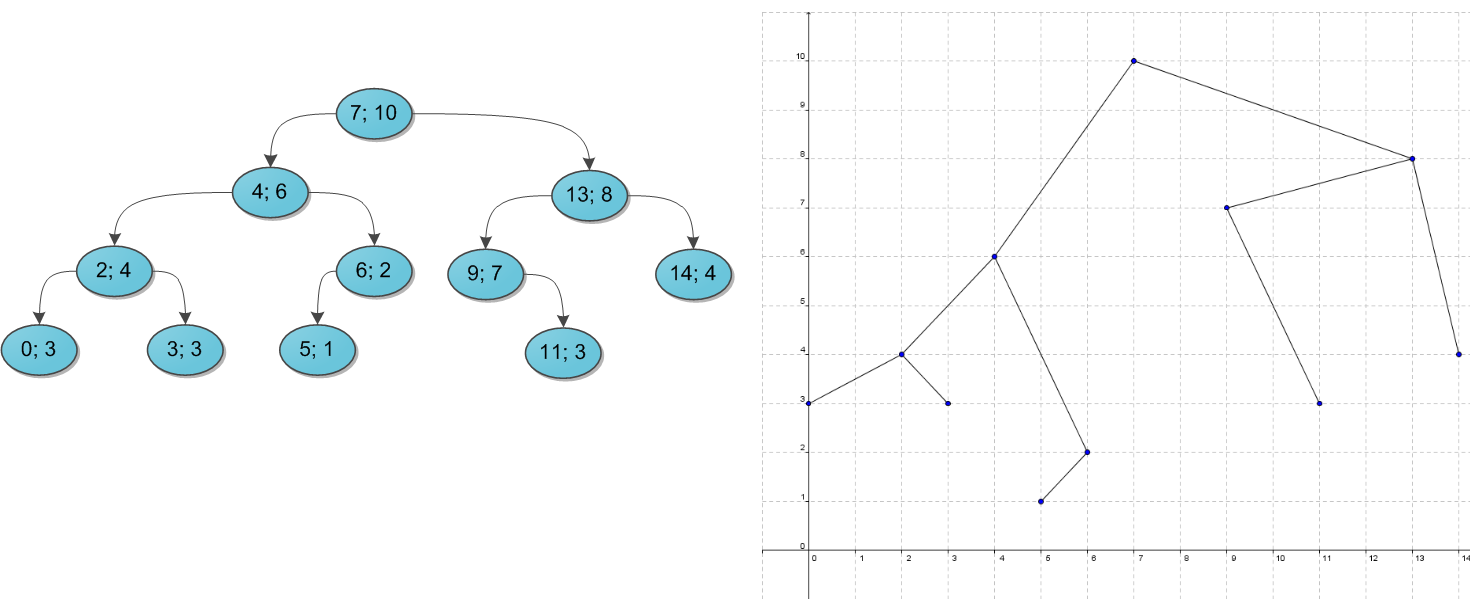
\includegraphics[scale=0.3]{treap.png}}
  \end{figure}
}

\subsection{Основные операции}
\frame
{
  \frametitle{Поиск, вставка и удаление}
  \begin{itemize}
    \item Поиск по ключу делается так же, как и в обычном дереве поиска.
    \item Вставка:
      \begin{itemize}
         \item вставляем в лист, как в обычном дереве
         \item может нарушиться свойство пирамиды для приоритетов
         \item нужно выполнить некоторое количество поворотов: не нарушают свойства дерева, но могут восстановить пирамиду для приоритетов.
       \end{itemize}
     \item Удаление:
       \begin{itemize}
         \item если удаляемый узел --- лист, освободить память,
         \item в противном случае, с помощью поворотов сделать узел листом.
       \end{itemize}
  \end{itemize}
}

\frame
{
  \frametitle{Пример}
  \begin{figure}[h!]
  \centerline{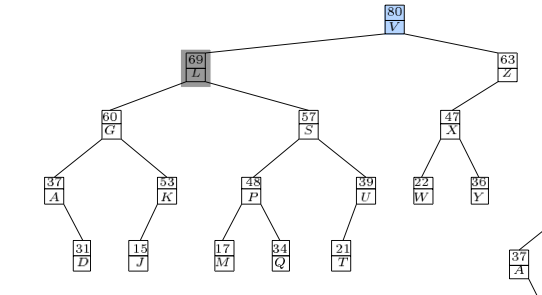
\includegraphics[scale=0.5]{ins1.png}}
  \end{figure}
}

\frame
{
  \frametitle{Пример}
  \begin{figure}[h!]
  \centerline{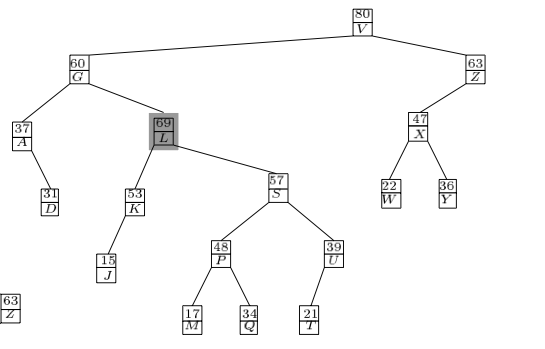
\includegraphics[scale=0.5]{ins2.png}}
  \end{figure}
}

\frame
{
  \frametitle{Пример}
  \begin{figure}[h!]
  \centerline{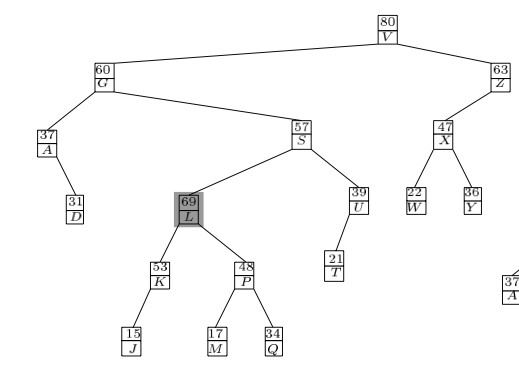
\includegraphics[scale=0.5]{ins3.png}}
  \end{figure}
}

\frame
{
  \frametitle{Пример}
  \begin{figure}[h!]
  \centerline{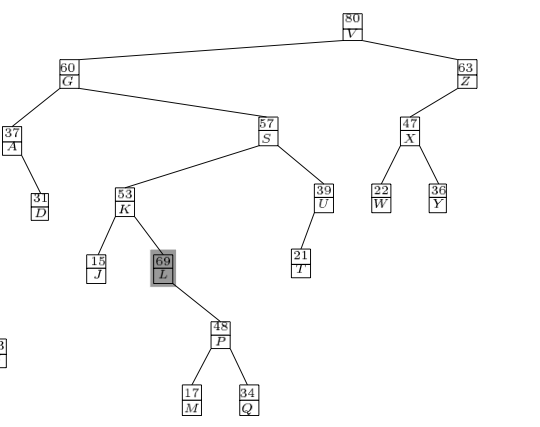
\includegraphics[scale=0.5]{ins4.png}}
  \end{figure}
}

\frame
{
  \frametitle{Пример}
  \begin{figure}[h!]
  \centerline{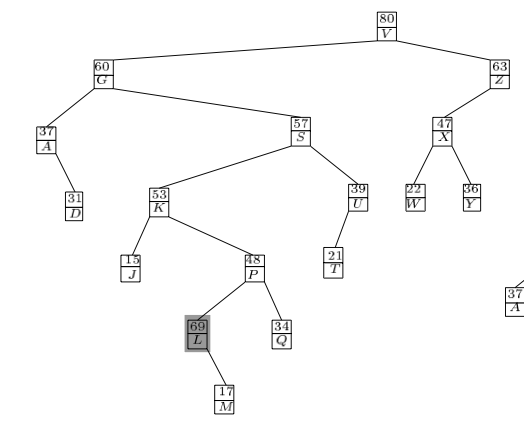
\includegraphics[scale=0.5]{ins5.png}}
  \end{figure}
}

\frame
{
  \frametitle{Пример}
  \begin{figure}[h!]
  \centerline{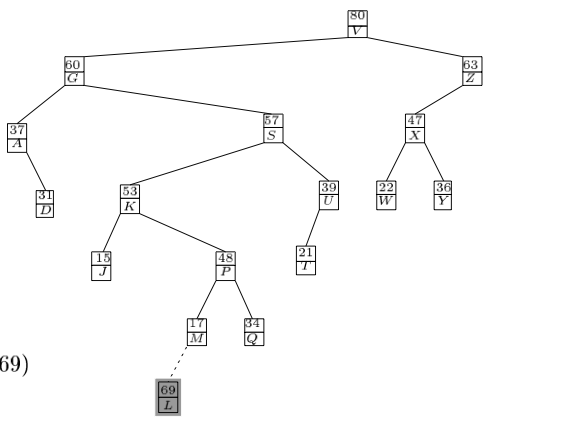
\includegraphics[scale=0.5]{ins6.png}}
  \end{figure}
}

\frame
{
  \frametitle{Реализация вставки}
  \begin{figure}[h!]
  \centerline{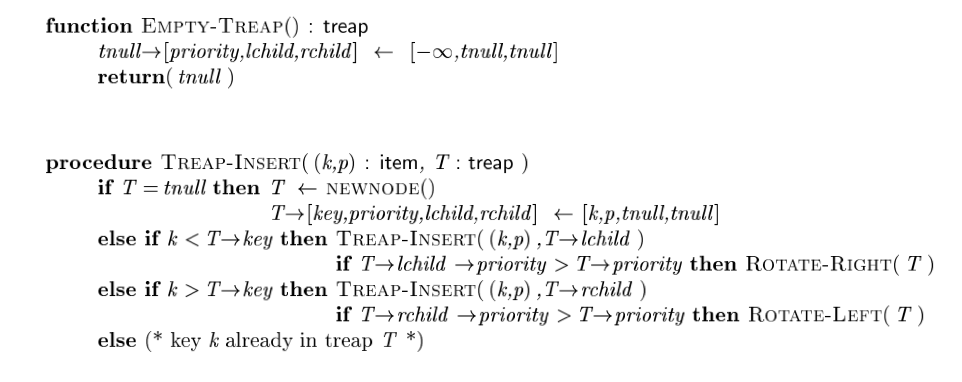
\includegraphics[scale=0.37]{ins-algo.png}}
  \end{figure}
}

\frame
{
  \frametitle{Реализация удаления}
   \begin{figure}[h!]
  \centerline{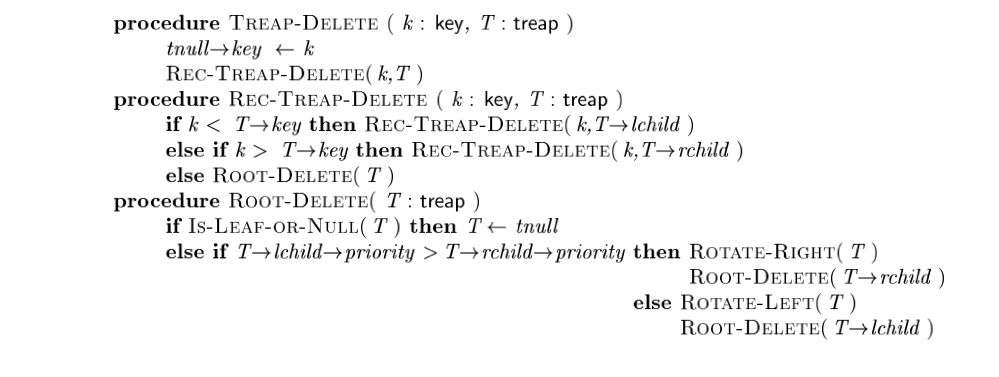
\includegraphics[scale=0.4]{del-algo.png}}
  \end{figure}
} 

\frame
{
  \frametitle{Разбиение и слияние}
  \begin{itemize}
    \item Если необходимо разбирть дерево на два по ключу k (в первом все ключи меньшие k, во втором~--- большие), можно добавить элемент $(k, \infty)$.
    \item Если нужно объединить два поддерева, можно сделать их сыновьями корня $(any, -\infty)$ и удалить корень.
    \item Обычно сначала реализуют операция разбиения и слияния, а через них~--- удаление и вставку.
  \end{itemize}
}

\subsection{Анализ времени работы}
\frame
{
\frametitle{Сложность доступа к случайному элементу}
 \begin{itemize}
   \item Дано декартово дерево, с элементами $x_1...x_n$, такими что $x_i.key < x_{i+1}.key$.
   \item $D(x)$~--- глубина узла $x$, количество узлов от $x$ до корня.
   \item $A_{i,j}$~--- характеристическая функция, равна 1, если $x_i$ предок $x_j$, иначе 0.
   \item $D(x_l) = \sum_{1 \leq i \leq n} A_{i, l}$.
   \item $E(A_{i,j}) = a_{i, j}$. Из линейности мат. ожидания $E(D(x_l)) = \sum_{1 \leq i \leq n} a_{i, l}$.
   \item $a_{i,j} = E(A_{i,j}) = Pr(A_{i,j} = 1) = Pr(ancestor(x_i, x_j))$
 \end{itemize}
}

\frame
{
\frametitle{Сложность доступа к случайному элементу}
\begin{itemize}
  \item $x_i$ будет предком $x_j$, тогда и только тогда, когда среди всех элементом от $i$ до $j$ $x_i$ имеет наибольший приоритет.
  \item Вероятность того, что $x_i$ предок $x_j$ при равномерном распределении приоритеров:
    $$
      a_{i,j} = \frac{1}{|i -j| + 1}
    $$
   \item Тогда: $E(D(x_l)) = H_l + H_{n+1-l} - 1 < 1 + 2\cdot\ln(n)$
\end{itemize}
}
 
\subsection{Неявные декартовы деревья}
\frame
{
\frametitle{Определение и применение}
   \begin{itemize}
   \item Простая модификация обычных декартовых деревьев: неявным ключем будет индекс декущего элемента в массиве, построенном по отсотрированным элементам
   \item Что можно будет сделать за O(log n):
      \begin{itemize}
        \item Вставка в массив на любую позицию
        \item Удаление произольного элемента
        \item Сумма, min, max на произвольном подотрезке.
      \end{itemize}
  \end{itemize}
}

\frame
{
\frametitle{Детали}
  \begin{itemize}
    \item Хранить сам порядковый номер нерационально, придется пересчитывать O(n) элементов каждый раз.
    \item Будем хранить количество элементов в поддереве, тогда порядковый номер можно найти, спускаясь по дереву от корня.
    \item Теперь можно находить произвольные подотрезки и функции на них (поддерживая дополнительное значение в элементах).
  \end{itemize}
}

\end{document}

